\usepackage{bchart}

\section{Checksum Calculation}

In order to uniquely identify the files analyzed, and detect changes across runs, the Data Discovery Library must
perform some calculations on each file to generate a unique ID that is dependent on the content of the file.
Ideally these calculations are efficient and the generated IDs will have a low collision rate.

\subsection{Hashing, CRC and Checksum Algorithms}
Before deciding on the algorithm that will be used to generate the IDs, it's important to clear up the differences
between hashing, checksum and CRC algorithms.
These terms are often used interchangeably (e.g.\ the metadata generated by the library also uses the term \("\)hash\("\)
as a place-holder for the ID field)

Arguably, these operations achieve similar results, i.e.\ taking an unknown sized chunk of data, and reducing it into
a constant n-sized output value.
However, they are intended for different use cases.
The goal of a hashing algorithm is to create values that have low
collision rates, they are also often used for cryptographic applications (which is irrelevant for this project).
The low collision rates however comes at the cost of slower computation rates, compared to checksum algorithms.
The values generated by hashing algorithms are referred to as digests.

\newline

Checksum and Cyclic Redundancy Check Algorithms both aim to detect errors in the files.
Of course, by extension this
also means that files with minor changes are guaranteed to have different checksum values.
They usually have
faster computation rates compared to hashing algorithms due to their smaller sizes and lack of cryptographic concerns.
Naturally, the smaller checksum sizes do increase the chances of collisions.

The difference between CRC and checksum algorithms is the method of calculation.
CRCs are slower, but able to generate larger error runs.

\subsection{Collisions and the Birthday Problem}

Since the generated values, are meant to be used as unique identifier for files and to track changes of the files, it's important
to discuss collision rates. Figure ~\ref{fig:checksum_fig_1} shows the birthday problem in action.
Essentially, if there are 77163 files, by using a 32-bit checksum, the odds of a collision is 50%.

Therefore, there must be a careful balance between performance and coliision rates.

\begin{figure}[h]
    \centering
    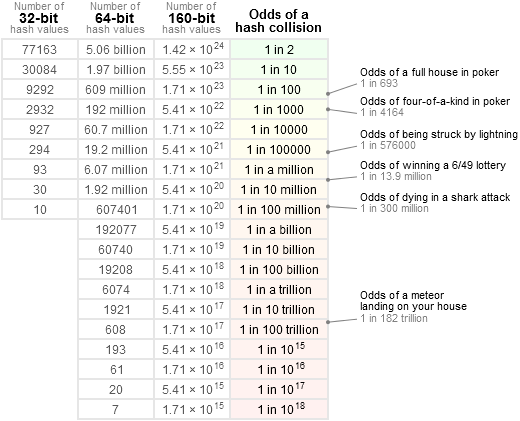
\includegraphics[width=12cm]{figures/checksum/collisions}
    \caption{Chances of collision for various bit sizes, source: ~\cite{PreshingCollisions}}
    \label{fig:checksum_fig_1}
\end{figure}



\subsection{Offloading the Hash Calculations into Compiled Modules}
Before investigating the various CRC and checksum algorithms.
It is beneficial to consider offloading the checksum calculations into a separate, compiled module.
It is easy to do so, since:

\begin{itemize}
    \item There isn't much interdependency between the checksum calculation and the rest of the library.
    \item The generated values are numeric, which are unlikely to cause conversion issues across the modules.
    \item Python has a well established culture, of offloading calculation heavy processes into compiled modules.
\end{itemize}

The checksum algorithms detailed below were all implemented in Rust.
Rust was chosen as it enables its users to write low level code, while still being memory safe.
Its performance is also comparable to C. That being said, the results here are reproducible on any compiled, low level
language, assuming it can interface with Python.

The modules were always compiled with the release flag on.
The python wheels were generated using Maturin ~\cite{Maturin}.

\begin{table}[]
\begin{tabular}{ll}
Operating System  & Ubuntu 22.04.1 LTS x86\_64                                     \\
Kernel Version    & 5.15.0-56                                                      \\
Processor         & Intel i7-4700MQ @ 3.400GHz                                     \\
Memory            & 16Gb DDR3 @ 1867MHz                                             \\
Hard drive        & SATA SSD @ 452.62 MB/s read                                    \\
Aggregate Size    & 50GB                                                           \\
File Distribution & 500 uniformly sized 100mb files containing output from urandom
\end{tabular}
\caption{Benchmark Environment}
\label{tab:checksum_tab_1}
\end{table}

The specifications of the benchmark environment are as shown on ~\ref{tab:checksum_tab_1}


\begin{bchart}[step=2,max=400]
    \bcbar[text=Year 1]{3.4}
        \smallskip
    \bcbar{5.6}
        \medskip
    \bcbar{7.2}
        \bigskip
    \bcbar{9.9}
\end{bchart}